% !TeX spellcheck = ru_RU
\documentclass[a4paper,12pt]{extarticle}
\usepackage[utf8x]{inputenc}
\usepackage[T1,T2A]{fontenc}
\usepackage[russian]{babel}
\usepackage{hyperref}
\usepackage{indentfirst}
\usepackage{listings}
\usepackage{color}
\usepackage{here}
\usepackage{array}
\usepackage{multirow}
\usepackage{graphicx}

\usepackage{caption}
\renewcommand{\lstlistingname}{Программа} % заголовок листингов кода

\bibliographystyle{ugost2008ls}

\usepackage{listings}
\lstset{ %
extendedchars=\true,
keepspaces=true,
language=C,						% choose the language of the code
basicstyle=\footnotesize,		% the size of the fonts that are used for the code
numbers=left,					% where to put the line-numbers
numberstyle=\footnotesize,		% the size of the fonts that are used for the line-numbers
stepnumber=1,					% the step between two line-numbers. If it is 1 each line will be numbered
numbersep=5pt,					% how far the line-numbers are from the code
backgroundcolor=\color{white},	% choose the background color. You must add \usepackage{color}
showspaces=false				% show spaces adding particular underscores
showstringspaces=false,			% underline spaces within strings
showtabs=false,					% show tabs within strings adding particular underscores
frame=single,           		% adds a frame around the code
tabsize=2,						% sets default tabsize to 2 spaces
captionpos=t,					% sets the caption-position to top
breaklines=true,				% sets automatic line breaking
breakatwhitespace=false,		% sets if automatic breaks should only happen at whitespace
escapeinside={\%*}{*)},			% if you want to add a comment within your code
postbreak=\raisebox{0ex}[0ex][0ex]{\ensuremath{\color{red}\hookrightarrow\space}},
texcl=true,
inputpath=listings,                     % директория с листингами
}

\usepackage[left=2cm,right=2cm,
top=2cm,bottom=2cm,bindingoffset=0cm]{geometry}

%% Нумерация картинок по секциям
\usepackage{chngcntr}
\counterwithin{figure}{section}
\counterwithin{table}{section}

%%Точки нумерации заголовков
\usepackage{titlesec}
\titlelabel{\thetitle.\quad}
\usepackage[dotinlabels]{titletoc}

%% Оформления подписи рисунка
\addto\captionsrussian{\renewcommand{\figurename}{Рисунок}}
\captionsetup[figure]{labelsep = period}

%% Подпись таблицы
\DeclareCaptionFormat{hfillstart}{\hfill#1#2#3\par}
\captionsetup[table]{format=hfillstart,labelsep=newline,justification=centering,skip=-10pt,textfont=bf}

%% Путь к каталогу с рисунками
\graphicspath{{fig/}}

\usepackage{minted}

\begin{document}	% начало документа

% Титульная страница
\begin{titlepage}	% начало титульной страницы

	\begin{center}		% выравнивание по центру

		\large Санкт-Петербургский политехнический университет Петра Великого\\
		\large Институт компьютерных наук и технологий \\
		\large Кафедра компьютерных систем и программных технологий\\[6cm]
		% название института, затем отступ 6см
		
		\huge Телекоммуникационные технологии\\[0.5cm] % название работы, затем отступ 0,5см
		\large Отчет по лабораторной работе №6\\[0.1cm]
		\large Цифровая модуляция\\[5cm]

	\end{center}


	\begin{flushright} % выравнивание по правому краю
		\begin{minipage}{0.25\textwidth} % врезка в половину ширины текста
			\begin{flushleft} % выровнять её содержимое по левому краю

				\large\textbf{Работу выполнил:}\\
				\large Графов Д.И.\\
				\large {Группа:} 33531/2\\
				
				\large \textbf{Преподаватель:}\\
				\large Богач Н.В.

			\end{flushleft}
		\end{minipage}
	\end{flushright}
	
	\vfill % заполнить всё доступное ниже пространство

	\begin{center}
	\large Санкт-Петербург\\
	\large \the\year % вывести дату
	\end{center} % закончить выравнивание по центру

\thispagestyle{empty} % не нумеровать страницу
\end{titlepage} % конец титульной страницы

\vfill % заполнить всё доступное ниже пространство


% Содержание
\setcounter{page}{2}
% Содержание
\renewcommand\contentsname{\centerline{Содержание}}
\tableofcontents
\newpage




\section{Цель работы}
Изучение методов модуляции цифровых сигналов.

\section{Программа работы}
\begin{enumerate}
	\item Получить сигналы BPSK, PSK, OQPSK, genQAM, MSK, M-FSK модуляторов.
	\item Построить их сигнальные созвездия.
	\item Провести сравнение изученных методов модуляции цифровых сигналов.
	
\end{enumerate}

\section{Теоретическая информация}
Модуляция (лат. modulatio — размеренность, ритмичность) — процесс изменения одного или нескольких параметров модулируемого несущего сигнала при помощи модулирующего сигнала.

В цифровой модуляции аналоговый несущий сигнал модулируется цифровым битовым потоком.
Существуют три фундаментальных типа цифровой модуляции (или шифтинга) и один гибридный:
\begin{itemize}
	\item ASK – Amplitude shift keying (Амплитудная двоичная модуляция).
	\item FSK – Frequency shift keying (Частотая двоичная модуляция).
	\item PSK – Phase shift keying (Фазовая двоичная модуляция).
	\item ASK/PSK.
\end{itemize}

В случае амплитудного шифтинга амплитуда сигнала для логического нуля может быть (например) в два раза меньше логической единицы.

Частотная модуляция похожим образом представляет логическую единицу интервалом с большей частотой, чем ноль.

Фазовый шифтинг представляет «0» как сигнал без сдвига, а «1» как сигнал со сдвигом.

Каждая из схем имеет свои сильные и слабые стороны.
\begin{itemize}
	\item ASK хороша с точки зрения эффективности использования полосы частот, но подвержена искажениям при наличии шума и недостаточно эффективна с точки зрения потребляемой мощности.
	\item FSK – с точностью до наоборот, энергетически эффективна, но не эффективно использует полосу частот.
	\item PSK – хороша в обоих аспектах.
	\item ASK/PSK – комбинация двух схем. Она позволяет еще лучше использовать полосу частот.
\end{itemize}

Самая простая PSK схема (показанная на рисунке) имеет собственное название — Binary phase-shift keying. Используется единственный сдвиг фазы между «0» и «1» — 180 градусов, половина периода.

Существуют также QPSK и 8-PSK:

QPSK использует 4 различных сдвига фазы (по четверти периода) и может кодировать 2 бита в символе (01, 11, 00, 10). 8-PSK использует 8 разных сдвигов фаз и может кодировать 3 бита в символе. 

Одна из частных реализаций схемы ASK/PSK которая называется QAM — Quadrature Amplitude Modulation (квадратурная амплитудная модуляция (КАМ). Это метод объединения двух AM-сигналов в одном канале. Он позваляет удвоить эффективную пропускную способность. В QAM используется две несущих с одинаковой частотой но с разницей в фазе на четверть периода (отсюда и возникает слово квадратура). Более высокие уровни QAM строятся по тому же принципы, что и PSK.

\newpage
\section{Ход выполнения работы}
Данная работа выполнялась с помощью библиотеки GNURadio.

GNU Radio — программный инструментарий, предоставляющий разработчикам программно-определяемых радиосистем «строительные блоки», обеспечивающие основные функции цифровой обработки сигналов.

Чтобы познакомиться с видами цифровой модуляции, были созданы 3 блок-схемы.

Приведём изображение одной из них в интерфейсе программы GNURadio.

Основне различие между ними - блок, следующий за Random Source - моделирующий.

\begin{figure}[H]
	\begin{center}
		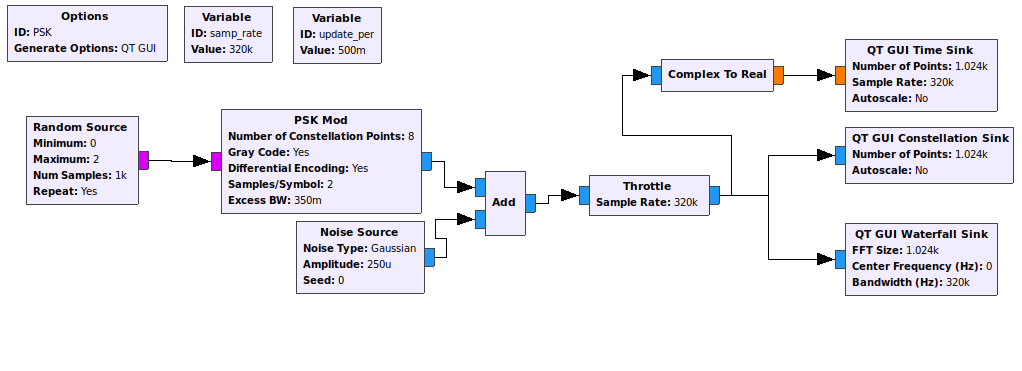
\includegraphics[width=\linewidth]{pics/GNURadio}
		\caption{Интерфейс GNURadio}
		\label{fig:GNURadio}
	\end{center}
\end{figure}

\newpage
\section{Результаты работы}

\begin{figure}[!htb]
	\minipage{0.32\textwidth}
	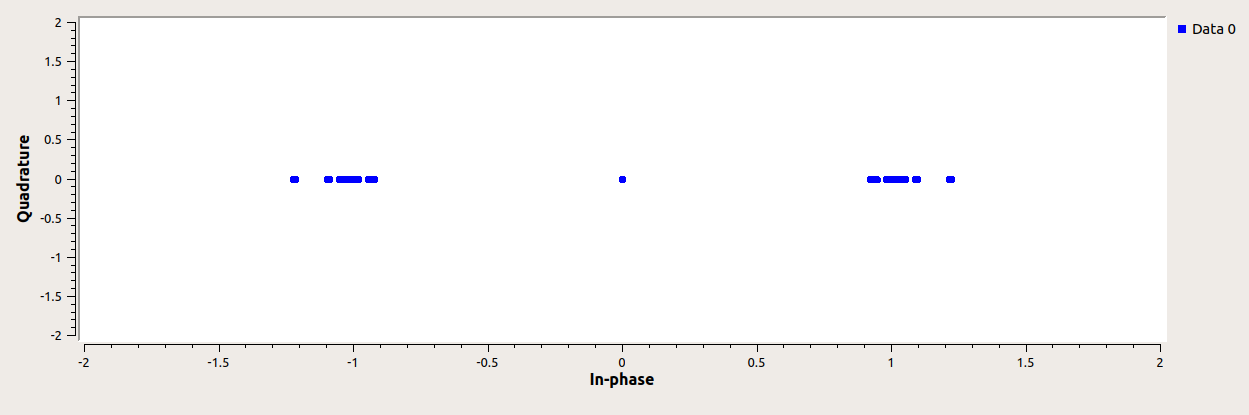
\includegraphics[width=\linewidth]{pics/BPSK}
	\caption{BPSK}\label{fig:BPSK}
	\endminipage\hfill
	\minipage{0.32\textwidth}
	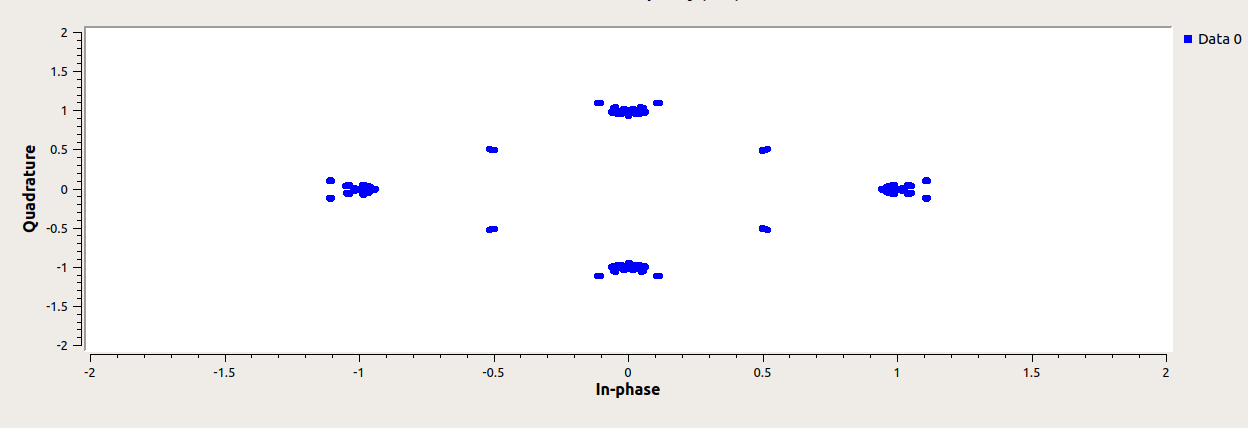
\includegraphics[width=\linewidth]{pics/QPSK}
	\caption{QPSK}\label{fig:QPSK}
	\endminipage\hfill
	\minipage{0.32\textwidth}%
	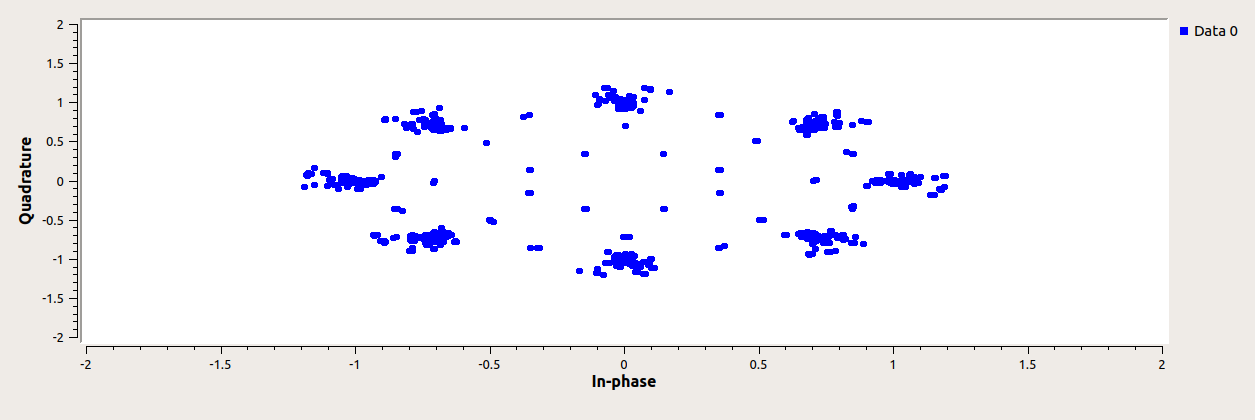
\includegraphics[width=\linewidth]{pics/8-PSK}
	\caption{8-PSK}\label{fig:8-PSK}
	\endminipage
\end{figure}

\begin{figure}[!htb]
	\minipage{0.5\textwidth}
	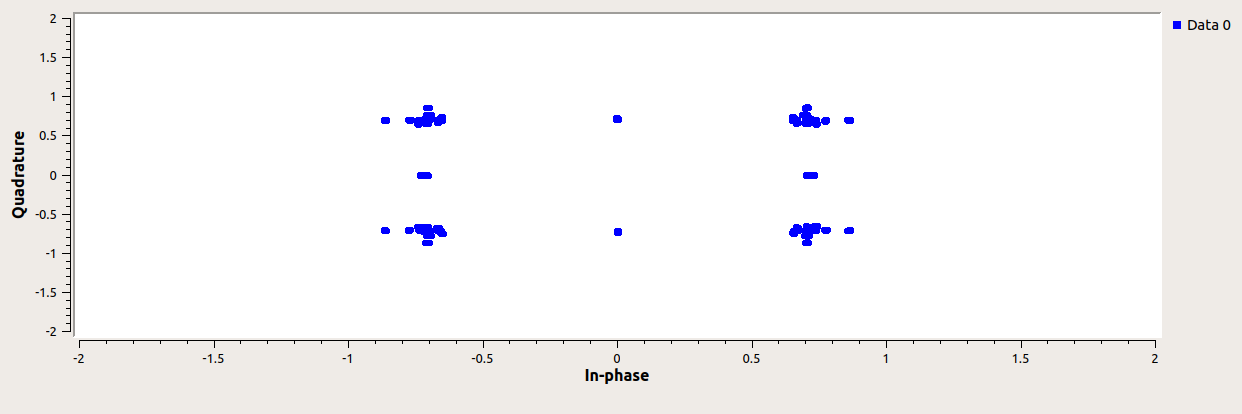
\includegraphics[width=\linewidth]{pics/QAM-4}
	\caption{QAM-4}\label{fig:QAM-4}
	\endminipage\hfill
	\minipage{0.5\textwidth}
	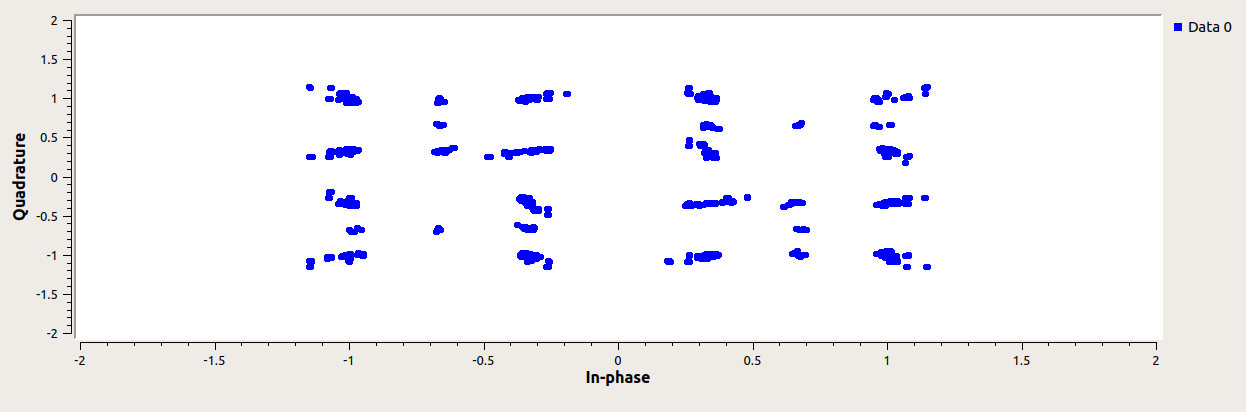
\includegraphics[width=\linewidth]{pics/QAM-16}
	\caption{QAM-16}\label{fig:QAM-16}
	\endminipage\hfill
\end{figure}

\begin{figure}[H]
	\begin{center}
		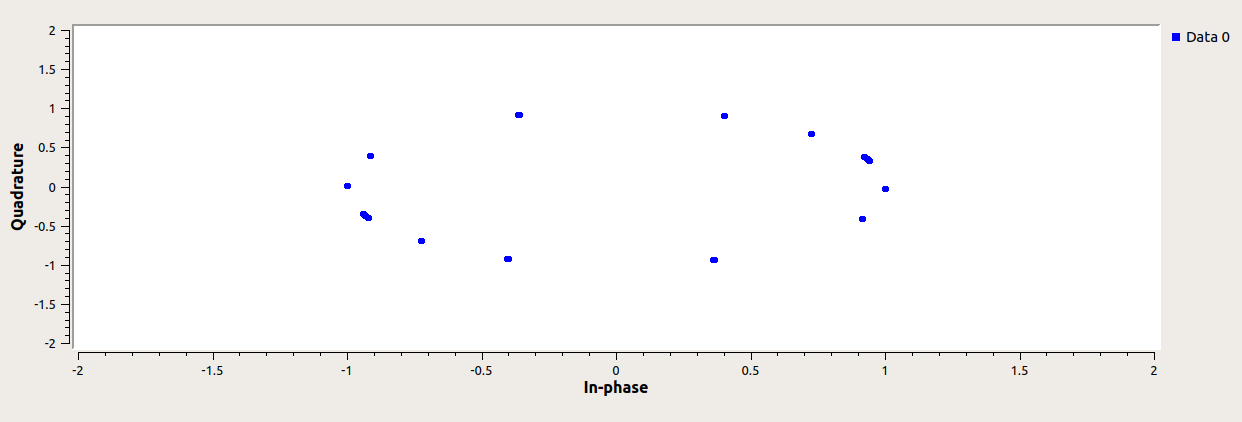
\includegraphics[width=\linewidth]{pics/GMSK}
		\caption{GMSK}
		\label{fig:GMSK}
	\end{center}
\end{figure}

\begin{figure}[!htb]
	\minipage{1\textwidth}
	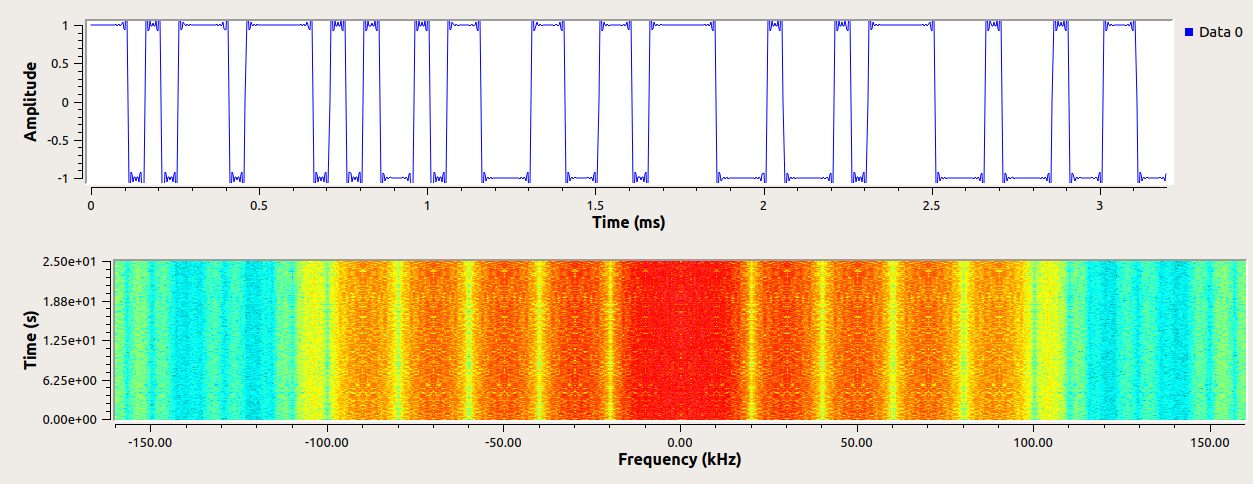
\includegraphics[width=\linewidth]{pics/BPSK_SIG}
	\caption{BPSK signal}\label{fig:BPSK}
	\endminipage\hfill
\end{figure}
\begin{figure}[!htb]
	\minipage{1\textwidth}
	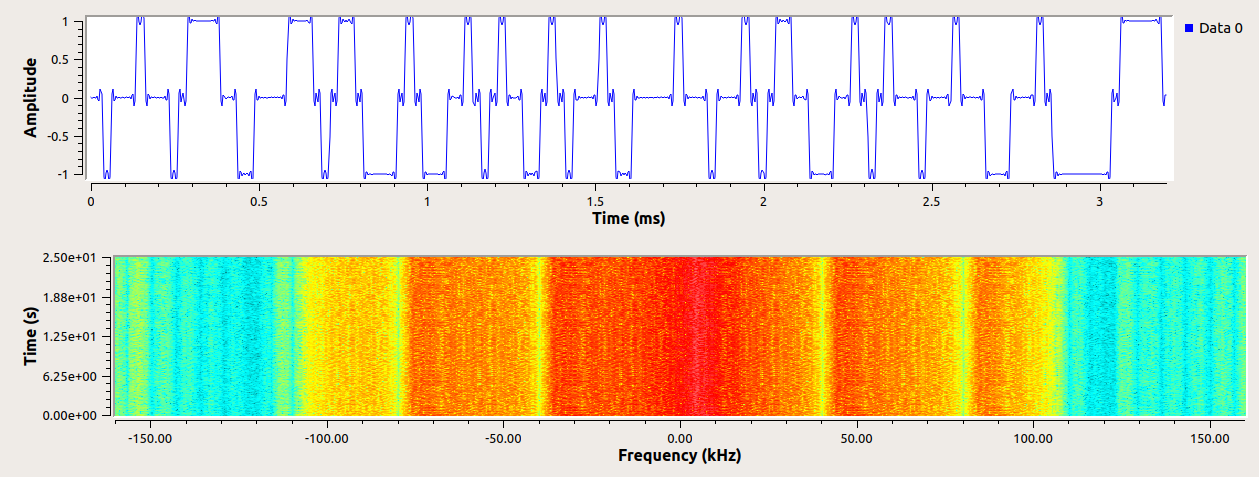
\includegraphics[width=\linewidth]{pics/QPSK_SIG}
	\caption{QPSK signal}\label{fig:QPSK}
	\endminipage\hfill
\end{figure}
\begin{figure}[!htb]
	\minipage{1\textwidth}%
	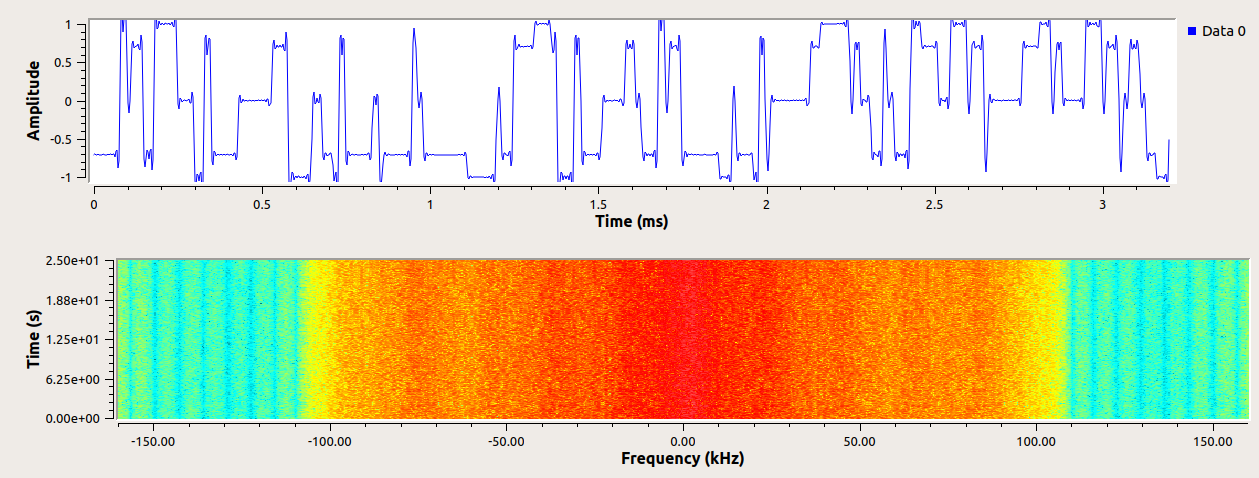
\includegraphics[width=\linewidth]{pics/8-PSK_SIG}
	\caption{8-PSK signal}\label{fig:8-PSK}
	\endminipage
\end{figure}

\begin{figure}[!htb]
	\minipage{1\textwidth}
	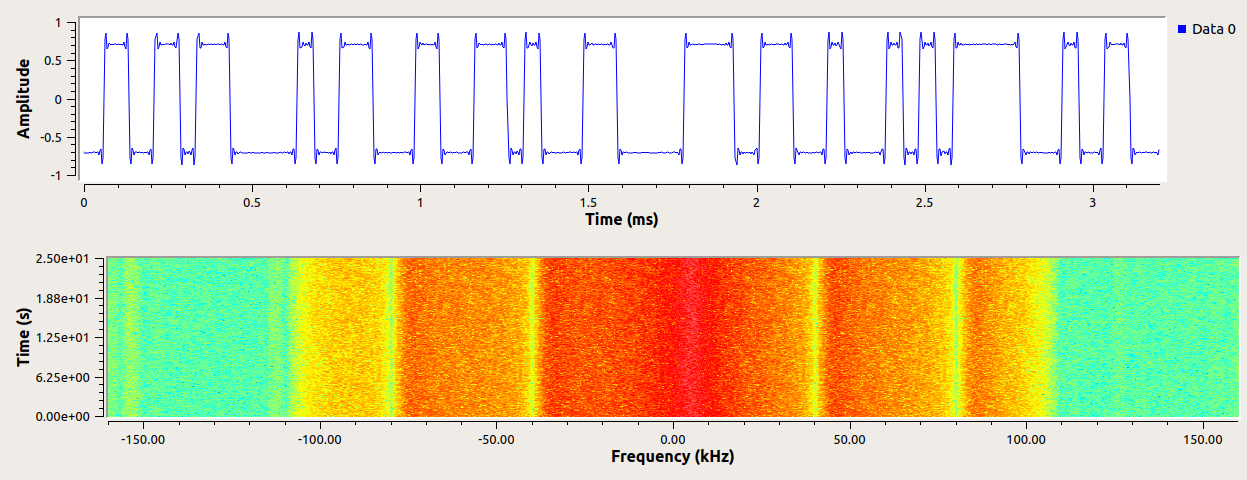
\includegraphics[width=\linewidth]{pics/QAM-4_SIG}
	\caption{QAM-4 signal}\label{fig:QAM-4}
	\endminipage\hfill
\end{figure}
\begin{figure}[!htb]
	\minipage{1\textwidth}
	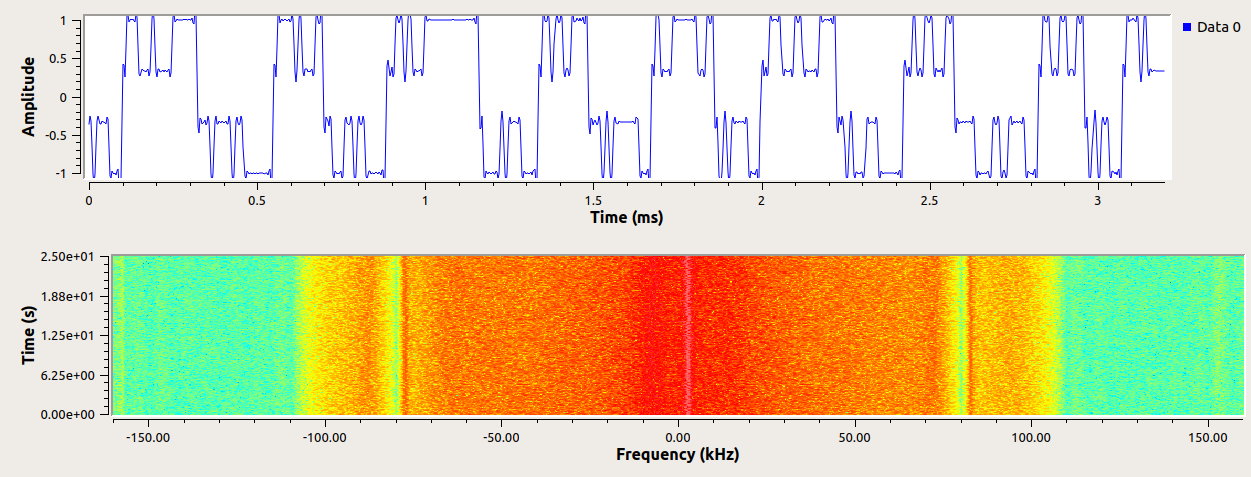
\includegraphics[width=\linewidth]{pics/QAM-16_SIG}
	\caption{QAM-16 signal}\label{fig:QAM-16}
	\endminipage\hfill
\end{figure}

\begin{figure}[!htb]
	\begin{center}
		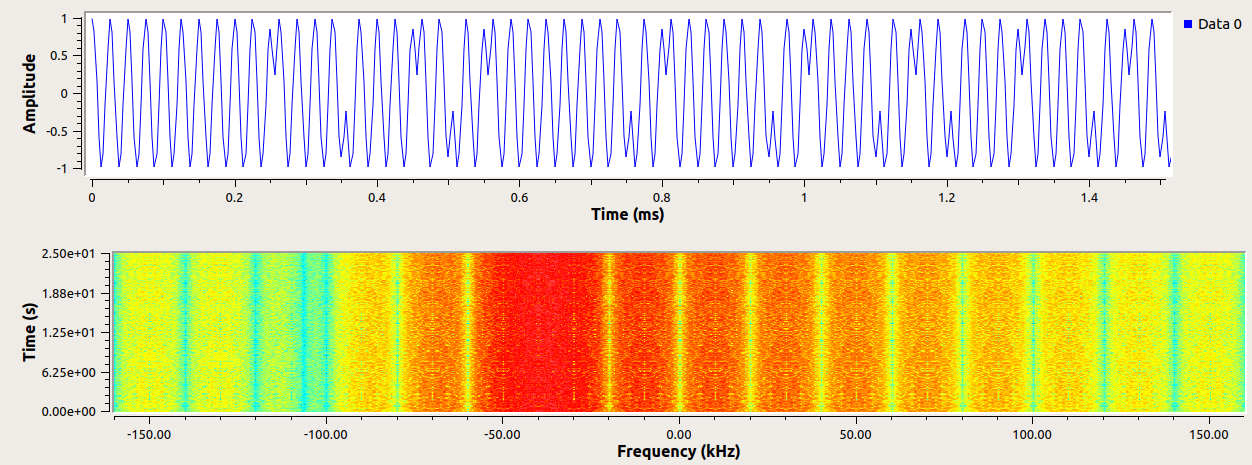
\includegraphics[width=\linewidth]{pics/GMSK-SIG}
		\caption{GMSK signal}
		\label{fig:GMSK}
	\end{center}
\end{figure}

Гауссовская частотная модуляция с минимальным сдвигом (англ. Gaussian Minimum Shift Keying (GMSK)) — вид частотой модуляции (манипуляции) с индексом модуляции равным 0.5, при которой последовательность из прямоугольных информационных импульсов проходит через гауссовский фильтр нижних частот.

Преимущество данного вида модуляции в том, что сигналы с GMSK имеют высокую скорость спада уровня внеполосных излучений, то есть меньше мешают другим пользователям эфира, чем сигналы с MSK. Как и сигналы с MSK, сигналы с GMSK имеют непрерывную фазу.

\newpage
\section{Выводы}
В ходе выполнения работы я ознакомился c основными возможностями библиотеки GNURadi. В рамках базовых возможностей библиотки были продемонстрированы основные виды цифровой модуляции.

Из полученных спектральных созвездий можно сделать вывод, что: 
\begin{itemize}
	\item Чем сложнее схема модуляции, тем более пагубное воздействие на нее оказывают искажения при передаче, и тем меньше расстояние от базовой станции, на котором сигнал может быть успешно принят.
	
	\item Теоретически возможны PSK и QAM схемы еще более высокого уровня, но на практике при их использовании возникает слишком большое количество ошибок.
\end{itemize}

\end{document}
